%! TEX program = xelatex

% loading packages; we rely on elsevier's template to load most packages
\documentclass{cas-dc} % elsevier's double-column class; it also loads many packages for us
\usepackage[utf8]{inputenc} % not required in newer compiler, but just in case
\usepackage[T1]{fontenc} % for 8bit font encoding
\usepackage[backend=biber, style=apa]{biblatex} % bibliography
\usepackage{setspace} % makes life easier when changing line spacing ...
\usepackage{gensymb}
\usepackage{threeparttable}
\usepackage{mathtools}

% the journal requires manuscripts to use 1.5 line spacing
%\onehalfspacing

% a hack that disables the email/url graphic logo prefix
\ExplSyntaxOn
\keys_set:nn {stm/mktitle} {nologo}
\ExplSyntaxOff

% a hack to replace natbib with biblatex when using cas-dc and cas-sc classes
\makeatletter
\newlength{\bibsep}{\@listi \global\bibsep\itemsep \global\advance\bibsep by\parsep}
\makeatother

% bibliography configuration (for biblatex)
\ExecuteBibliographyOptions{sorting=none, sortcites=true, sortsets=true}
\ExecuteBibliographyOptions{dashed=false, hyperref=true, isbn=false, url=false, doi=true}
\urlstyle{same} % fix the font of url and doi in bibliography
\addbibresource{reference.bib} % use only one single bib file

% prefix section number to equation indices
\numberwithin{equation}{section}

% default figure search path
\graphicspath{{../figs/}}

% priority of the formats of figures
\DeclareGraphicsExtensions{.pdf,.png}

% custom commands; aliases
\newrobustcmd*{\geoclaw}{\texttt{GeoClaw}\xspace} % monospace text for GeoClaw
\newrobustcmd*{\geoclawlandspill}{\texttt{GeoClaw-landspill}\xspace} % monospace text for GeoClaw-landspill
\newrobustcmd*{\vectorsym}[1]{\mathbfit{#1}} % vector symbols
\renewrobustcmd*{\vec}{\vectorsym} % use vector symbols instead of arrow for vec
\newrobustcmd*{\mat}[1]{\mathbfit{#1}} % matrix symbols
\newrobustcmd*{\diff}{\mathop{}\!\mathup{d}} % ISO-style upright ordinary differentiation
\newrobustcmd*{\pd}[3][1]{\ifstrequal{#1}{1}{\frac{\partial #2}{\partial #3}}{\frac{\partial^{#1} #2}{\partial #3^{#1}}}} % partial derivative

% document body
\begin{document}

% front matter
%! TEX root = main.tex

% title
\title[mode=title]{(TBD) Modeling oil overland flow in pipeline rupture events using shallow-water equations}

% authorship
\author[1]{Pi-Yueh Chuang}[orcid=0000-0001-6330-2709]
\ead{pychuang@gwu.edu}

\author[2]{Tracy Thorleifson}
\ead{Tracy.Thorleifson@g2-is.com }

\author[1]{Lorena A. Barba}[orcid=0000-0001-5812-2711]
\cormark[1] 

\cortext[cor1]{Corresponding author. \textit{Email address:} \texttt{labarba@gwu.edu}}
\ead[url]{https://lorenabarba.com/}

\address[1]{Department of Mechanical and Aerospace Engineering, The George Washington University, Washington, DC, USA}
\address[2]{G2 Integrated Solutions, Houston, TX 77042, USA}

% abstract; not sure why we need [S U M M A R Y]
\begin{abstract}[S U M M A R Y]
    This is a place holder.
    This is a place holder.
    This is a place holder.
    This is a place holder.
    This is a place holder.
    This is a place holder.
    This is a place holder.
    This is a place holder.
    This is a place holder.
    This is a place holder.
    This is a place holder.
    This is a place holder.
    This is a place holder.
    This is a place holder.
    This is a place holder.
    This is a place holder.
    This is a place holder.
    This is a place holder.
    This is a place holder.
    This is a place holder.
    This is a place holder.
    This is a place holder.
\end{abstract}

% keywords
\begin{keywords}
    oil overland flow \sep
    pipeline \sep
    shallow-water equarions
\end{keywords}

% vim:ft=tex

\maketitle

% sections
\section{Introduction} \label{sec:introduction}
    %! TEX root = main.tex

In the US, between 2010 and 2017, an average of 388 hazardous liquid pipeline accidents happened per year.
50\% of accidents contaminate soil, and 41\% of accidents affect areas with high consequences in either ecology or economy.
Moreover, 85\% on average of the released oil was not recovered and kept damaging the environment (\cite{belvederesi_statistical_2018}).
From the perspective of risk management, while pipelines are unavoidable in modern days, it is necessary to understand how a pipeline may impact the environment if any accidental release happens.
\geoclawlandspill serves this purpose.
\geoclawlandspill provides a free and open-source simulation tool to researchers investigating the danger, risk, and loss posted by potential pipeline accidents.

To our knowledge, \geoclawlandspill is the only open-source high-fidelity flow simulator for oil pipeline rupture events.
High fidelity means the results provide more details and accuracy because of high-resolution digital elevation data, fine spatial discretization, and full shallow-water equations.
Commercial products with a similar capability to \geoclawlandspill are available \cite{Zuczek2008, RPSGroup, Hydronia, Gin2012}.
Other non-commercial software more or less serving a similar purpose usually relies on simplified models, such as 1D open-channel models, diffusive wave approximation, gravity current models, and gradient-based route selection models \cite{Hussein2002, Simmons2003, Ronnie2004, farrar_gis_2005, Guo2006, Su2017}.
Moreover, these non-commercial codes are either non-exist in modern days or are not open-source.

Another value of \geoclawlandspill is to provide a platform for scholars who study oil flow modeling to implement and test their models.
As the main flow solver is under the BSD 3-Clause License, scholars can add their models to *geoclaw-landspill* freely.

SWE has been used to model overland flow problems such as rainfall-runoff problems, dam-break problems, tsunami simulations, and river flow simulations.
One major difference between oil overland flow and the aforementioned applications lies in the rheological properties of the working fluids.



\section{Governing equations and models} \label{sec:methods}
    %! TEX root = main.tex
\subsection{Full shallow-water equations}

We model the oil overland flow with the full shallow-water equations (SWE), which are derived from depth-averaged Navier-Stokes equations (\cite{vreugdenhil_numerical_1994}):
\begin{equation}\label{eq:swe}
    \pd{}{t}\vec{q} + \pd{}{x}\vec{f}(\vec{q}) + \pd{}{y}\vec{g}(\vec{q}) = \vec{\psi}(\vec{q}, x, y, t)
\end{equation}
where $\vec{q} = \begin{bmatrix} h \\ hu \\ hv \end{bmatrix}$,
$\vec{f}(\vec{q}) = \begin{bmatrix} hu \\ hu^2 + \frac{1}{2}gh^2 \\ huv \end{bmatrix}$,
$\vec{g}(\vec{q}) = \begin{bmatrix} hv \\ huv \\ hv^2 + \frac{1}{2}gh^2 \end{bmatrix}$, and
$\vec{\psi}(\vec{q}, x, y, t) = \begin{bmatrix} R-I \\ -ghB_x - F_x \\ -ghB_y - F_y \end{bmatrix}$.
Table \ref{table:notation} describes the meaning of each symbol.

\begin{table}
    \caption{Notation}
    \begin{tabular*}{\linewidth}[t]{p{0.11\linewidth}p{0.06\linewidth}p{0.7\linewidth}}
        \toprule
        Symbol & Unit & Description \\
        \midrule
        $x$, $y$ & $m$ & Spatial coordinates. \\
        $t$ & $s$ & Temporal coordinates. \\
        $g$ & $m/s^2$ & Gravitational acceleration. \\
        $h$ & $m$ & Fluid depth. \\
        $u$, $v$ & $m/s$ & Depth-averaged velocity in $x$- and $y$-directions. \\
        $R$, $I$ & $m/s$ & Mass source and sink. \\
        $B_x$, $B_y$ & none & Gradient components of topography in $x$- and $y$-directions. \\
        $F_x$, $F_y$ & $m^2/s^2$ & Bottom friction components in $x$- and $y$-directions. \\
        \bottomrule
    \end{tabular*}
    \label{table:notation}
\end{table}

Shallow-water equations are derived under the assumption of incompressible flow and Newtonian fluids. 
Though not all hydrocarbon products are Newtonian fluids, crude oils normally are. (\cite{Ronningsen2012, bryan_viscosity_2002}) 
In this work, our main focus is the crude oil pipelines. 

Equation \ref{eq:swe} is also called the dynamic shallow-water equations because it considers the effects of local acceleration, inertia, pressure, gravity, and viscosity.
While many variants and simplified shallow-water equations exist, we argue that the full shallow-water equations are necessary to describe the overland flow in pipeline incidents.
The gravity effect takes place everywhere because of topographical changes.
The pressure effect also applies to everywhere as long as the water surface elevation is not horizontal.
The inertia is at least significant at the vicinity of a pipeline rupture point and at the beginning of a rupture incident: the high pressure difference between inside and outside a pipe generates high flow speed at a rupture point.
Lastly, the viscosity effect is lumped into the bottom friction and is at least significant to flow front and after pipeline valves are shut down, causing flow speed to be slower.

George and Berger (\cite{George2011, Berger2011}) provide detailed descriptions of the numerical methods, especially the adaptive-mesh-refinement (AMR) algorithms, used in \geoclaw.
Built on top of \geoclaw, our work focuses on adding models for mass sources ($R$), mass sinks ($I$), bottom friction ($F_x$ and $F_y$), and temperature-dependent viscosity.
Our work also adds features that helps practical use cases in real-world analysis, such as standard CF-compliant NetCDF I/O, Esri ArcGIS integration, and cloud computing integration with Microsoft Azure.

    %! TEX root = main.tex

\subsection{Mass source: rupture points}

We model a rupture point with a point inflow source feeding fluid into the domain.
Oil leak rates are specified in $m^3/s$, while the mass source term ($I$) requires $m^2/s$.
We calculate the source term by dividing the actual flow rates with the grid cell area at each AMR level.
Though this approach is simple and robust in practice, theoretically speaking, its numerical stability is still unclear when combined with the AMR algorithms in \geoclaw.

The leak rates can be modeled with a three-stage constant profile.
First, at the beginning of an incident, the high pressure from the upstream causes a high flow rate.
The leak rate is almost a constant due to the upstream constant pressure.
Second, once the pipeline operator identifies the pipeline section containing the breaking location, the operator shuts down the valves controlling that section.
The remaining oil in that section keeps flowing out.
The rate at this stage, theoretically, decreases along with time because the pressure continues to decrease.
In this work, however, we still model this stage with a constant for model simplicity.
As the real rate profile at this stage depends on many factors (such as the types of breakage, fluid properties, or operation conditions), there may not be a single model that can apply to all types of rupture events.
Finally, after the oil in the affected section is completely drained out, or once the pressure in the pipeline is not high enough, the leak rate of the point source becomes zero.

Given a specific location of breakage, the time span and the flow rate of each stage may be estimated with model predictions (\cite{abhulimen_liquid_2004}) or, in common practice, rely on the inputs from field experts.
Figure \ref{fig:outflow-profile} shows an example profile 

\begin{figure}
    \centering
    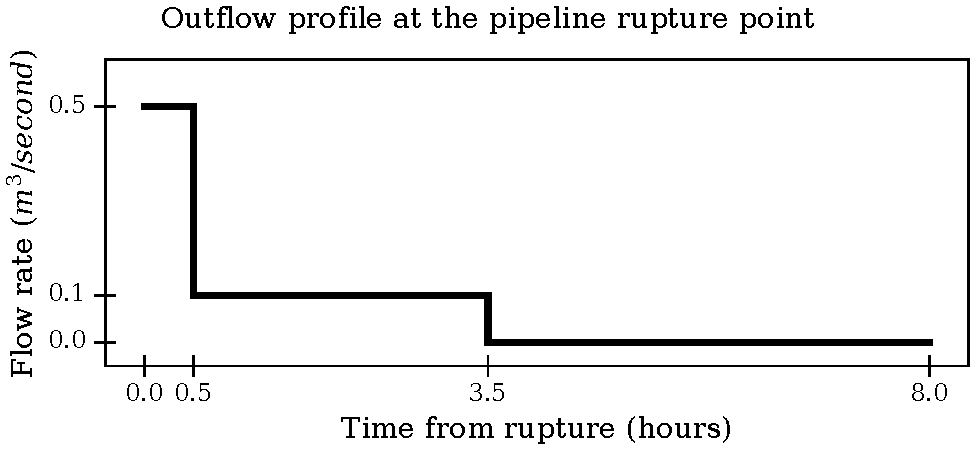
\includegraphics[width=0.9\linewidth]{landspill-outflow-profile}
    \caption{Outflow profile at the pipeline rupture point}\label{fig:outflow-profile}
\end{figure}

    %! TEX root = main.tex

\subsection{Mass sink: evaporation}


    %! TEX root = main.tex

\subsection{Mass sink: in-land waterbodies}


    %! TEX root = main.tex

\subsection{Darcy-Weisbach bottom friction}

Equation \ref{eq:swe} lumps viscosity effects into bottom friction forces ($F_x$ and $F_y$), which can be calculated with either the Manning equation or Darcy-Weisbach equation.
Manning equation and Darcy-Weisbach equation were originally developed for closed-pipe and open-channel flows. 
Practitioners also apply them to overland flow as they deem overland flow as infinite-width open-channel flow. (\cite{bellos_friction_2018})
Well-justified bottom friction models for overland flows, to the best of our knowledge, do not exist yet.

We implemented Darcy-Weisbach models for friction forces in our code. We will discuss why we prefer Darcy-Weisbach models over the Manning equation later in section \ref{sec:discussion}. The Darcy-Weisbach equation is:

\begin{equation}
    \begin{bmatrix} F_x \\ F_y \end{bmatrix}
    =
    \gamma(\boldsymbol{q})\begin{bmatrix} hu \\ hv \end{bmatrix}
    =
    \frac{f}{8h^2}\sqrt{(hu)^2+(hv)^2}\begin{bmatrix} hu \\ hv \end{bmatrix}
\end{equation}
$f$ is the Darcy-Weisbach coefficient.
Different Darcy-Weisbach models rely on different empirical equations to calculate the Darcy-Weisbach coefficient.

Our code support two different models (\cite{cheng_formulas_2008, bellos_friction_2018}) to calculate the Darcy-Weisbach coefficient. Figure \ref{fig:darcy-weisbach-models} shows the friction coefficients calculated using the two models under different surface roughness.

\begin{figure}
    \centering
    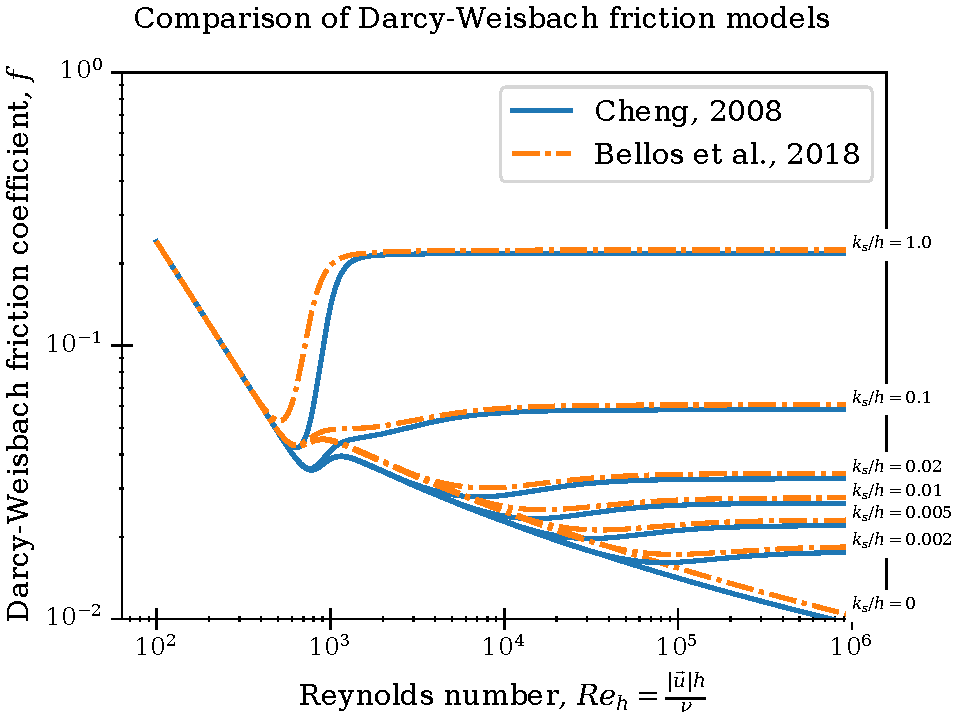
\includegraphics[width=0.9\linewidth]{darcy-weisbach-models}
    \caption{%
        Comparing the friction coefficients from the models in \cite{cheng_formulas_2008} and \cite{bellos_friction_2018} with different surface roughness $k_s$.
    }\label{fig:darcy-weisbach-models}
\end{figure}

\subsubsection{\cite{cheng_formulas_2008}}

Cheng proposed the following formula, which covers flow regimes from laminar to fully-rough turbulent flow:
\begin{equation}
    \begin{split}
        &\begin{multlined}
            f =
            \left( \frac{24}{Re_h} \right)^\alpha
            \times
            \left( 1.8\log_{10}\frac{Re_h}{2.1} \right)^{-2\left(1-\alpha\right)\beta}
            \\
            \times
            \left( 2\log_{10}\frac{11.8h}{k_s} \right)^{-2\left(1-\alpha\right)\left(1-\beta\right)}
        \end{multlined}\\
        &\alpha=\left[1+\left(\frac{Re_h}{850}\right)^9\right]^{-1}
        \text{, }
        \beta=\left[1+\left(\frac{Re_h k_s}{160h}\right)^2\right]^{-1}
    \end{split}
\end{equation}
$Re_h\equiv\frac{h\sqrt{u^2+v^2}}{\nu}$ is the Reynolds number defined with flow depth $h$ and kinematic viscosity $\nu$.
$k_s$ denotes the characteristic length of surface roughness. 

\subsubsection{\cite{bellos_friction_2018}}

Bellos, Nalbantis, and Tsakiris proposed an alternative formula for flood flow (we re-arranged it for clarity):
\begin{equation}
    \begin{split}
        &\begin{multlined}
            f =
            \left( \frac{24}{Re_h} \right)^\alpha
            \times
            \left( \frac{\sqrt{8}}{C_sRe_h}e^{1+W(\frac{\kappa}{e}C_sRe_h)} \right)^{2\left(1-\alpha\right)\beta}
            \\
            \times
            \left( \sqrt{8}\kappa\ln^{-1}(\frac{C_r}{e}\frac{h}{k_s}) \right)^{2\left(1-\alpha\right)\left(1-\beta\right)}
        \end{multlined} \\
        &\alpha=\left[1+\left(\frac{Re_h}{678}\right)^{8.4}\right]^{-1}
        \text{, }
        \beta=\left[1+\left(\frac{Re_h k_s}{150h}\right)^{1.8}\right]^{-1}.
    \end{split}
\end{equation}
$e$ and $\kappa\approx 0.4187$ denote Euler's number and the von Karman constant, respectively.
$C_s=8.94$ and $C_r=33.2$ are constants determined through fitting closed-pipe experimental data.
$W$ is an approximation to the Lambert W function: 
\begin{equation}
    \begin{multlined}
        W(x)
        =
        \ln(x)
        -
        \ln(\ln(x))
        +
        \frac{\ln(\ln(x))}{\ln(x)}
        \\
        +
        \frac{\ln^2(\ln(x))-2\ln(\ln(x))}{2\ln^2(x)}
    \end{multlined}
\end{equation}
This approximation has relative errors smaller than $0.1\%$ in the regime of smooth turbulent flow ($700 < Re_h < 25{,}000$).
Note this friction model, though designed for flood flow, is still based on 1D open-channel flow models and experimental data.

    %! TEX root = main.tex

\subsection{Temperature-dependent viscosity}



\section{Results: validations and showcases} \label{sec:results}
    %! TEX root = main.tex
\section{Results: validations and showcases}

\subsection{Regression test and validation: Malpasset dam-break problem}

We developed \geoclawlandspill{} by modifying and extending \geoclaw{}.
Whenever a simulation does not require any new functionalities, \geoclawlandspill{} should behave the same as \geoclaw{} does.
In this subsection we present a regression test to verify that our modifications do not introduce new bugs into the core SWE solver.
This test also serves as a validation test to the core SWE solver.

The Malpasset dam-break happened in southern France in 1959.
This incident has become a standard validation case for SWE solvers because of the detailed field survey data.
Figure \ref{fig:malpasset-topo-gauges} shows the digitalized elevation model (i.e., topography) and locations where we have real-world data.
We obtained the topography data from the validation package of Telemac-2D (\url{www.opentelemac.org}).
Points P1 to P17 on figure \ref{fig:malpasset-topo-gauges} indicate where the field survey data are available.
Points S6 to S14 indicate the gauge measurements from lab experiments on a scaled-model.
For the description and the coordinates of these data points, please refer to Biscarini et al. (\cite{biscarini_simulation_2016}).

\begin{figure}
    \centering
    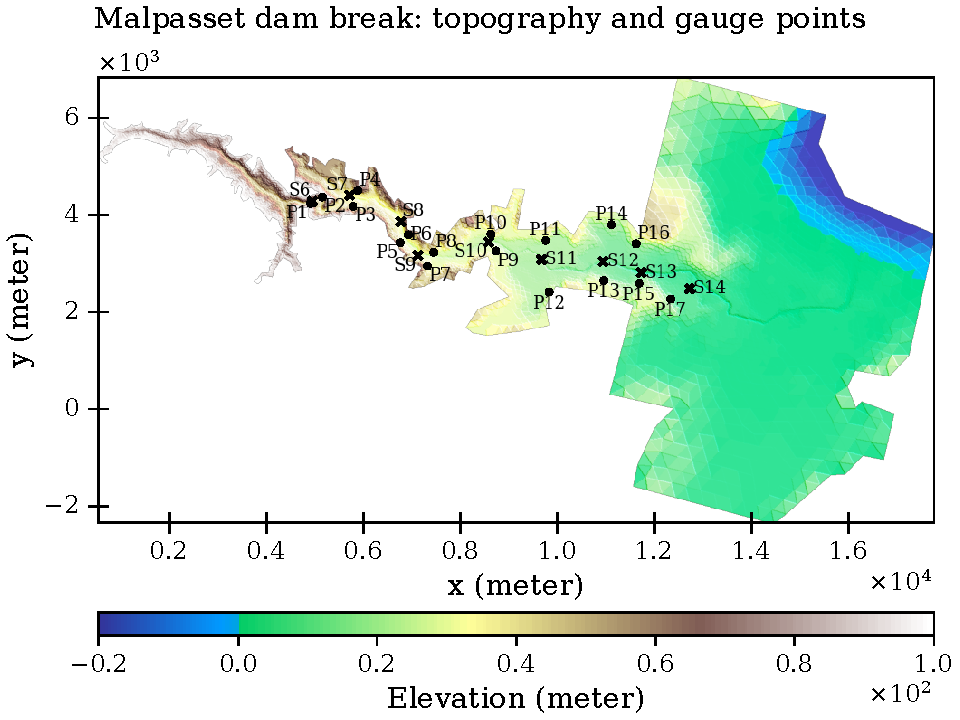
\includegraphics[width=0.9\linewidth]{malpasset-topo-gauges}
    \caption{Topography model and locations of gauges and field survey points}\label{fig:malpasset-topo-gauges}
\end{figure}

Figure \ref{fig:malpasset-gauge-field-survey} shows the maximum water surface levels at field survey locations.
Figure \ref{fig:malpasset-gauge-model} and figure \ref{fig:malpasset-arrival-time} show the maximum water surface levels and water arrival time at the scaled-model's gauges in the experiment.
We compared the simulation results from upstream \geoclaw{} and our \geoclawlandspill{} against the survey/experimental data.
We also compared against the result from GeoClaw in 2011 (\cite{George2011}).
The result from \geoclawlandspill{} agrees with that from upstream \geoclaw{}, which verifies that no bug was introduced.
The result from 2011 \geoclaw{}, however, has a slight discrepancy from our simulation results.
Compared to the field survey and the lab experiment, the simulation results have worse agreement with P1, P13, S6, and S9 on water surface level.
At gauge S14, the simulated arrival time deviates from the lab experiment.

\begin{figure}
    \centering
    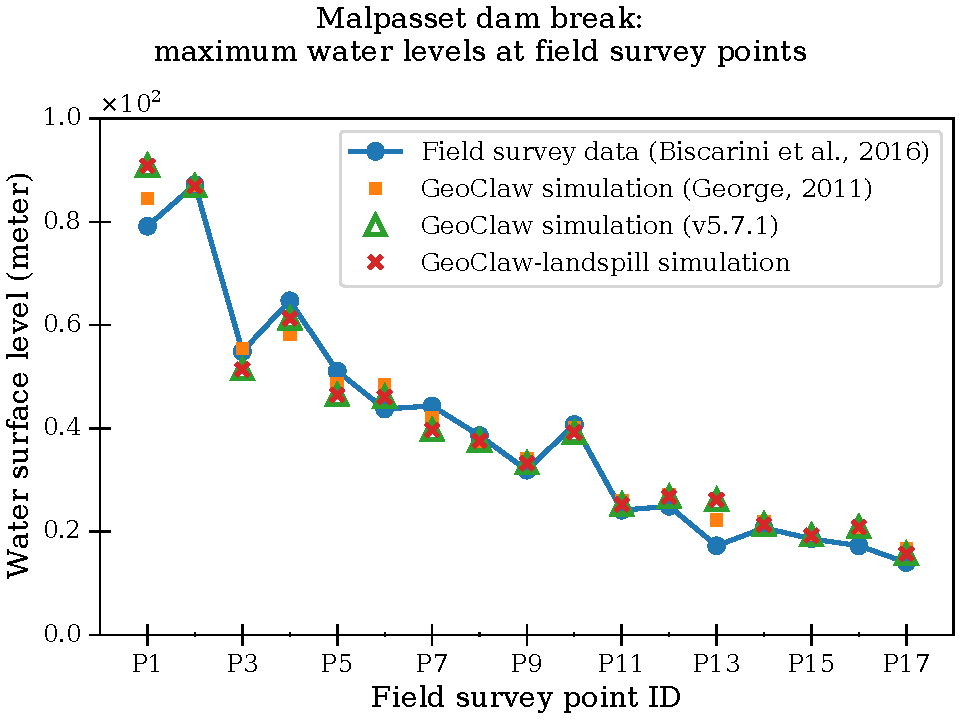
\includegraphics[width=0.9\linewidth]{malpasset-gauge-field-survey}
    \caption{Maximum water surface level at field survey locations}\label{fig:malpasset-gauge-field-survey}
\end{figure}

\begin{figure}
    \centering
    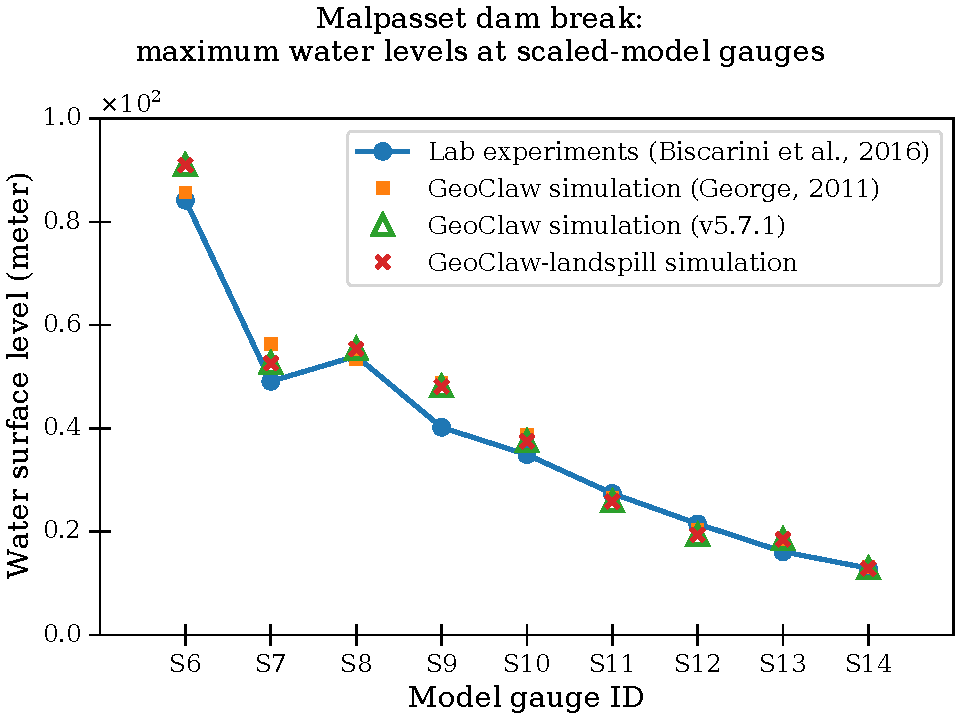
\includegraphics[width=0.9\linewidth]{malpasset-gauge-model}
    \caption{Maximum water surface level at scaled-model gauges}\label{fig:malpasset-gauge-model}
\end{figure}

\begin{figure}
    \centering
    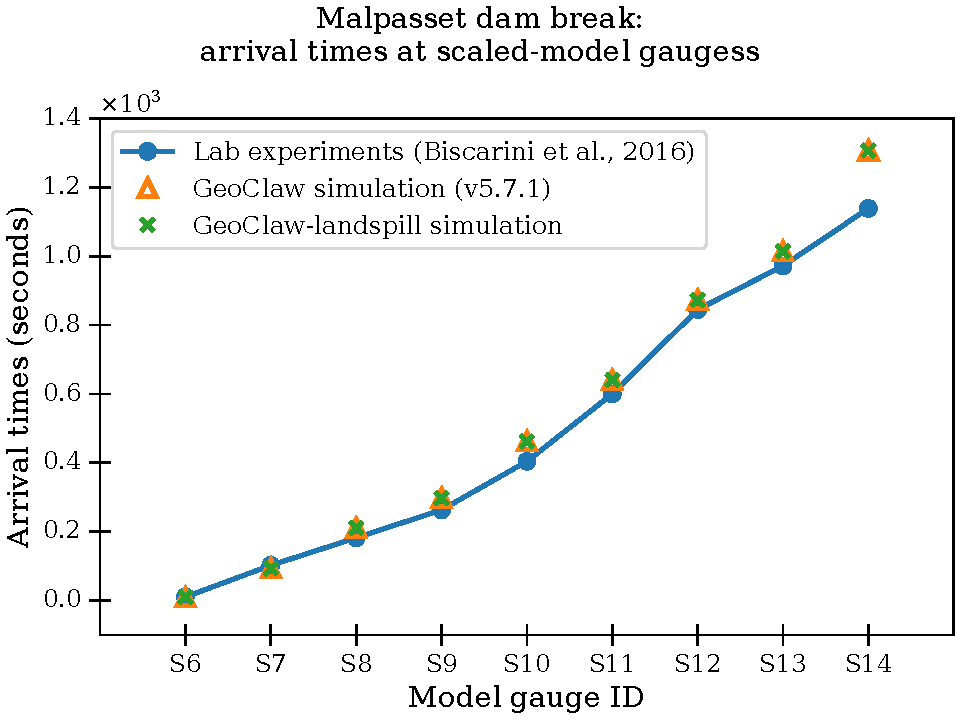
\includegraphics[width=0.9\linewidth]{malpasset-arrival-time}
    \caption{Water arrival times at scaled-model gauges}\label{fig:malpasset-arrival-time}
\end{figure}

\subsection{Validation: silicone oil on an inclined glass plate}

\begin{table}
    \caption{Viscosity ($\mu$), density ($\rho$) and evaporation coefficients ($C_1$ \& $C_2$) of the fluids}\label{table:fluid-properties}
    \begin{threeparttable}
        \begin{tabular*}{\tblwidth}{@{} LRRR@{} }
            \toprule
            & $\mu$ ($cP$) & $\rho$ ($kg/m^3$) & ($C_1$, $C_2$). \\
            \midrule
            Silicone    & 1096.1 & 970 & N/A \\
            Maya crude  & 322 & 926.6 & ($1.38$, $0.045$) \\
            Gasoline    & 0.6512 & 800 & ($13.2$, $0.21$) \\
            \bottomrule
        \end{tabular*}
        \begin{tablenotes}\footnotesize
            \item[*] Maya crude oil's and gasoline's properties are defined at 15\degree{} C.
                Silicone's properties are defined at an unknown temperature.
            \item[$\dagger$] References:~\cite{fingas_appendix_2015}.
        \end{tablenotes}
    \end{threeparttable}
\end{table}



\begin{figure*}
    \centering
    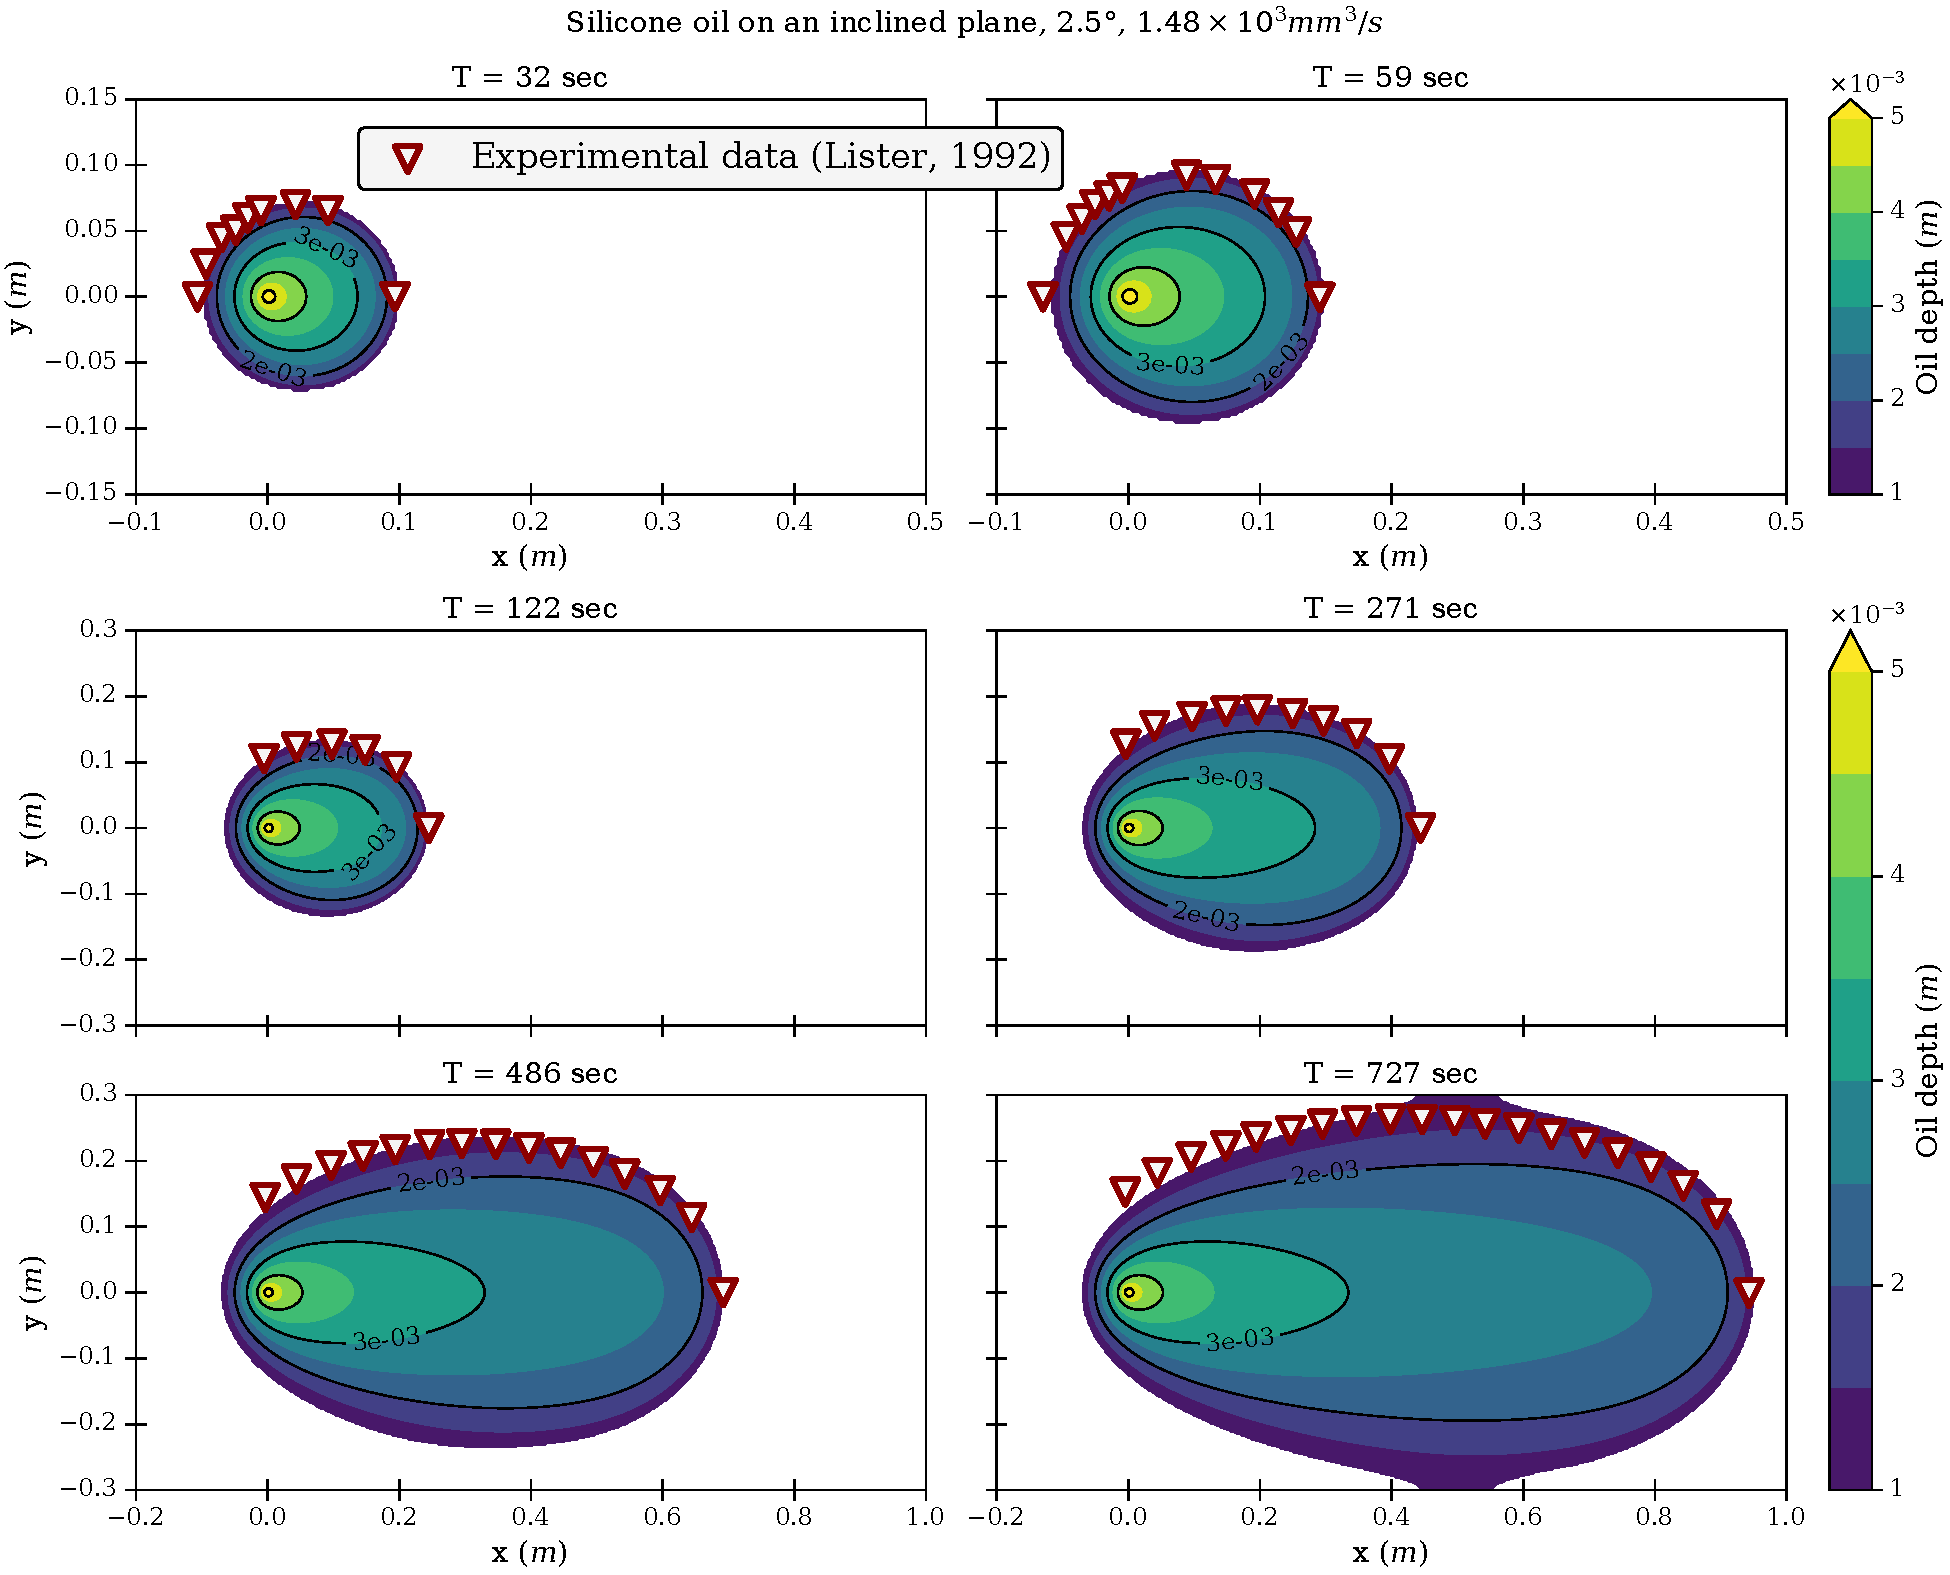
\includegraphics[width=\textwidth]{landspill-silicone-inclined-plane}
    \caption{%
        A validation case of silicone oil on an inclined plane: $angle=2.5\ \mathrm{\degree}$, $flow\ rate=1.48\times 10^{-6}\ \mathrm{m^3/s}$, $outflow\ location=(0, 0)$, $surface\ roughness=0\ \mathrm{m}$, and $ambient\ temperature=25\ \mathrm{\degree C}$. %
        The silicone oil have the following properties: $\mu=1096.1\ \mathrm{cP}$ at $25\ \mathrm{\degree C}$ and $\rho=970\ \mathrm{kg/m^3}$ at $15\ \mathrm{\degree C}$. %
        Note the difference in the coordinate scales in sub-figures. %
        Lister did not mention the flow thickness at the flow front. %
        In this simulation results, we use $1\times 10^{-3}\ \mathrm{m}$ to determine the flow front.%
    }\label{fig:landspill-silicone-inclined}
\end{figure*}

\subsection{Showcase: Maya crude oil and gasoline above flat terrain}

\begin{figure}
    \centering
    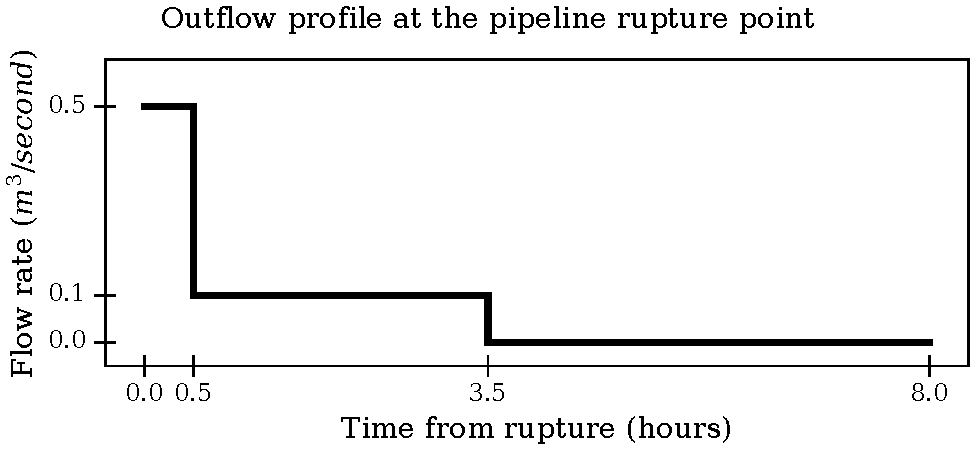
\includegraphics[width=0.9\linewidth]{landspill-outflow-profile}
    \caption{Outflow profile at the pipeline rupture point}\label{fig:outflow-profile}
\end{figure}

\begin{figure}
    \centering
    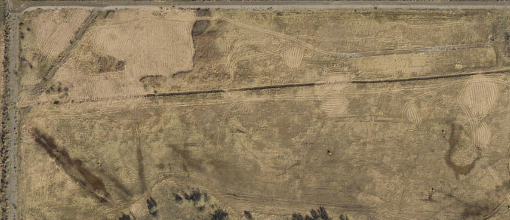
\includegraphics[width=0.9\linewidth]{flat}
    \caption{%
        A flat terrain near Salt Lake City, Utah. %
        Extent (left, bottom, right, top) in EPSG3857: $(-12459905, 4985865, -12459395, 4986085)$.
    }\label{fig:flat-terrain-satellite}
\end{figure}

\begin{figure*}
    \includegraphics[width=\textwidth]{landspill-maya-gasoline-flat-terrain}
    \caption{%
        Maya crude oil and gasoline above flat terrain near Salt Lake City, Utah. %
        The pipeline rupture point, i.e., the outflow location, is located close to the center of each plot. %
        Maya crude oil has higher viscosity than gasoline. %
        The flow, however, is not affected by the viscosity at the beginning stage, where the inertia dominates the flow due to the high outflow rate from the rupture point. %
        In later stages, the outflow rates becomes much smaller. %
        The evaporation rates start to play a much important role than the viscosity does. %
        Evaporation affects the volume of fluid above ground and then further affects the bottom friction, where the viscosity comes into play in SWEs.%
    }\label{fig:landspill-maya-gasoline-flat}
\end{figure*}

\subsection{Showcase: Maya crude oil in drainage terrain}

\begin{figure}
    \centering
    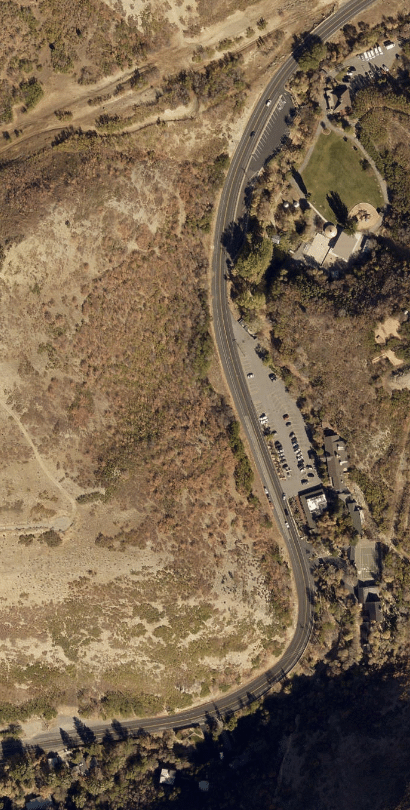
\includegraphics[width=0.7\linewidth]{hill}
    \caption{%
        A hill area near Salt Lake City, Utah. %
        Extent (left, bottom, right, top) in EPSG3857: $(-12443674, 4976959, -12443264, 4977769)$.
    }\label{fig:hill-terrain-satellite}
\end{figure}

\begin{figure*}
    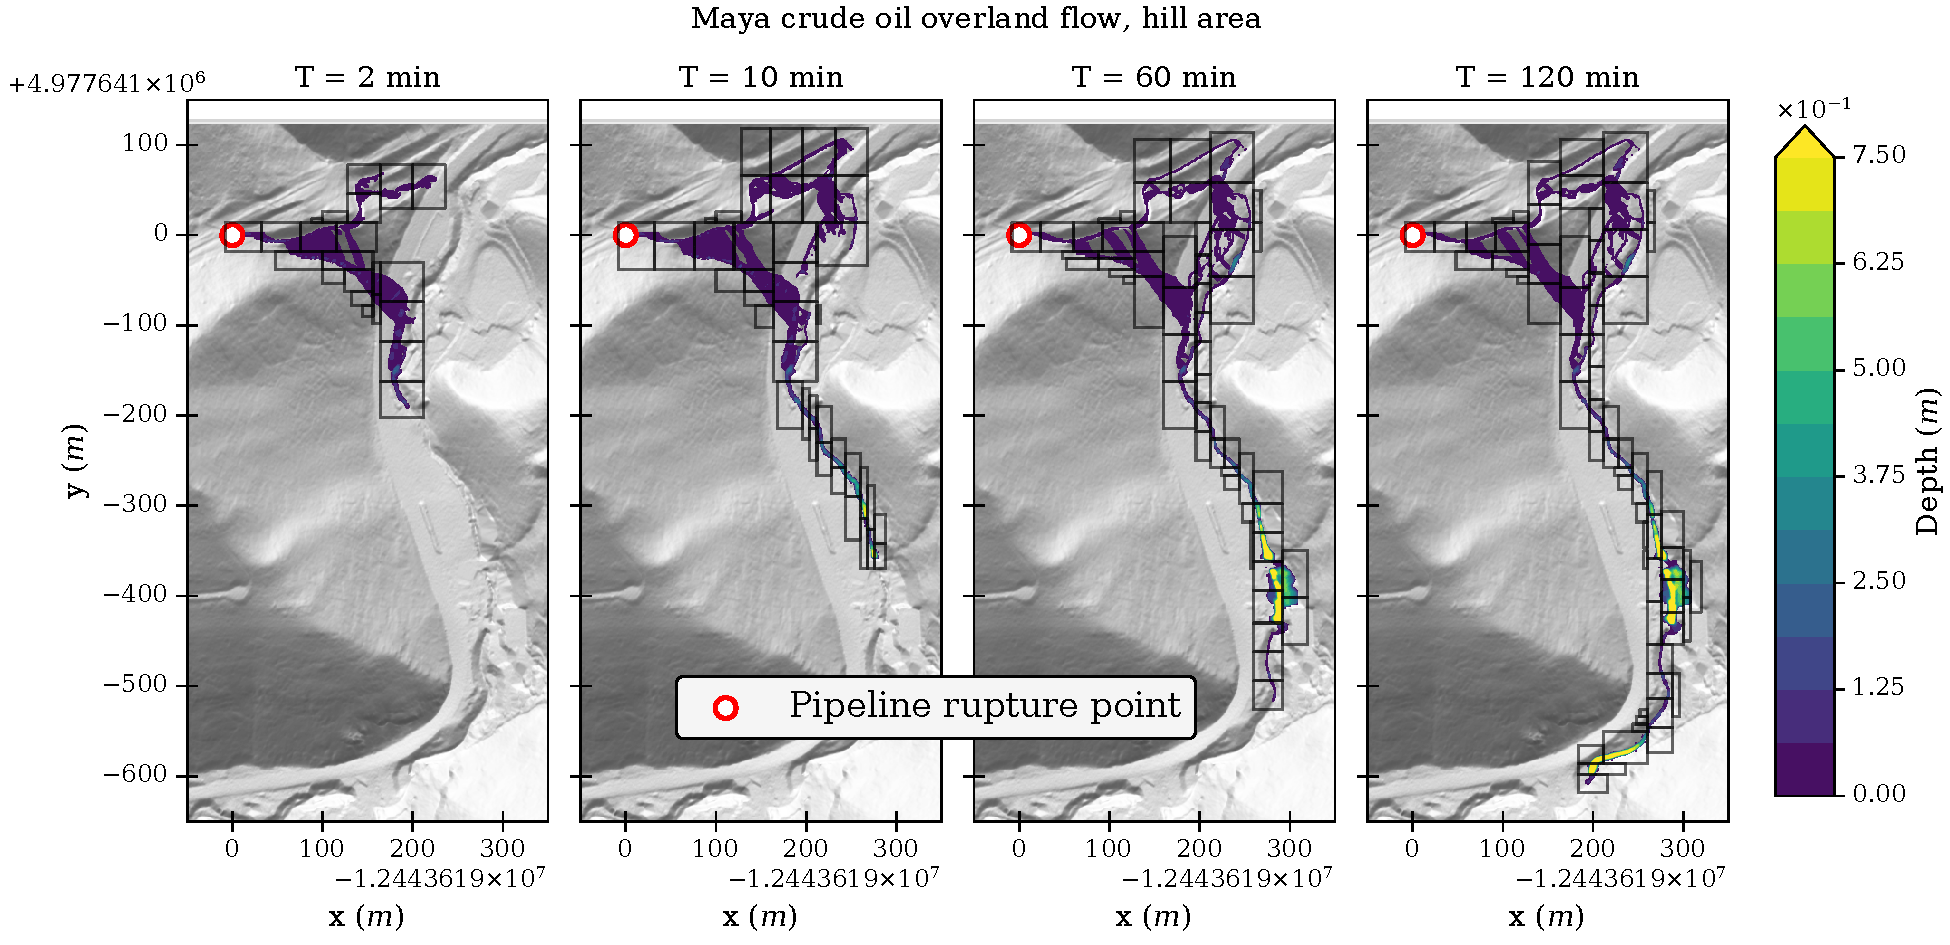
\includegraphics[width=\textwidth]{landspill-maya-hill}
    \caption{%
        Maya crude oil in a hill area near Salt Lake City, Utah. %
        The boxes shown in the figures indicate where the AMR high-resolution grid patches are. %
        In hill areas, flow patterns usually consist of thin but long streams. %
        Resolving the streams with Cartesian grids requires high-resolution grids everywhere in computational domains. %
        And simulations waste much computing power and time because the majority of the grid cells do not have fluid. %
        The use of AMR helps the calculation performance of this type of flows. %
        AMR applies high-resolution grid patches to regions with fluid, while dry regions still use low-resolution grids.%
    }\label{fig:landspill-maya-hill}
\end{figure*}

\subsection{showcase: Maya crude oil in contact with inland water bodies}

\begin{figure}
    \centering
    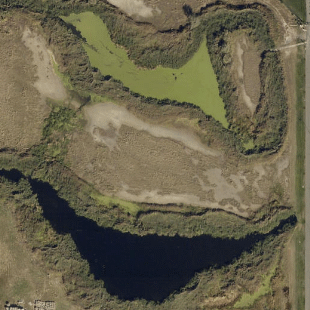
\includegraphics[width=0.7\linewidth]{hydro}
    \caption{%
        An area near Salt Lake City, Utah that has an in-land water body. %
        Extent (left, bottom, right, top) in EPSG3857: $(-12460364, 4984982, -12460054, 4985292)$.
    }\label{fig:hydro-terrain-satellite}
\end{figure}

\begin{figure*}
    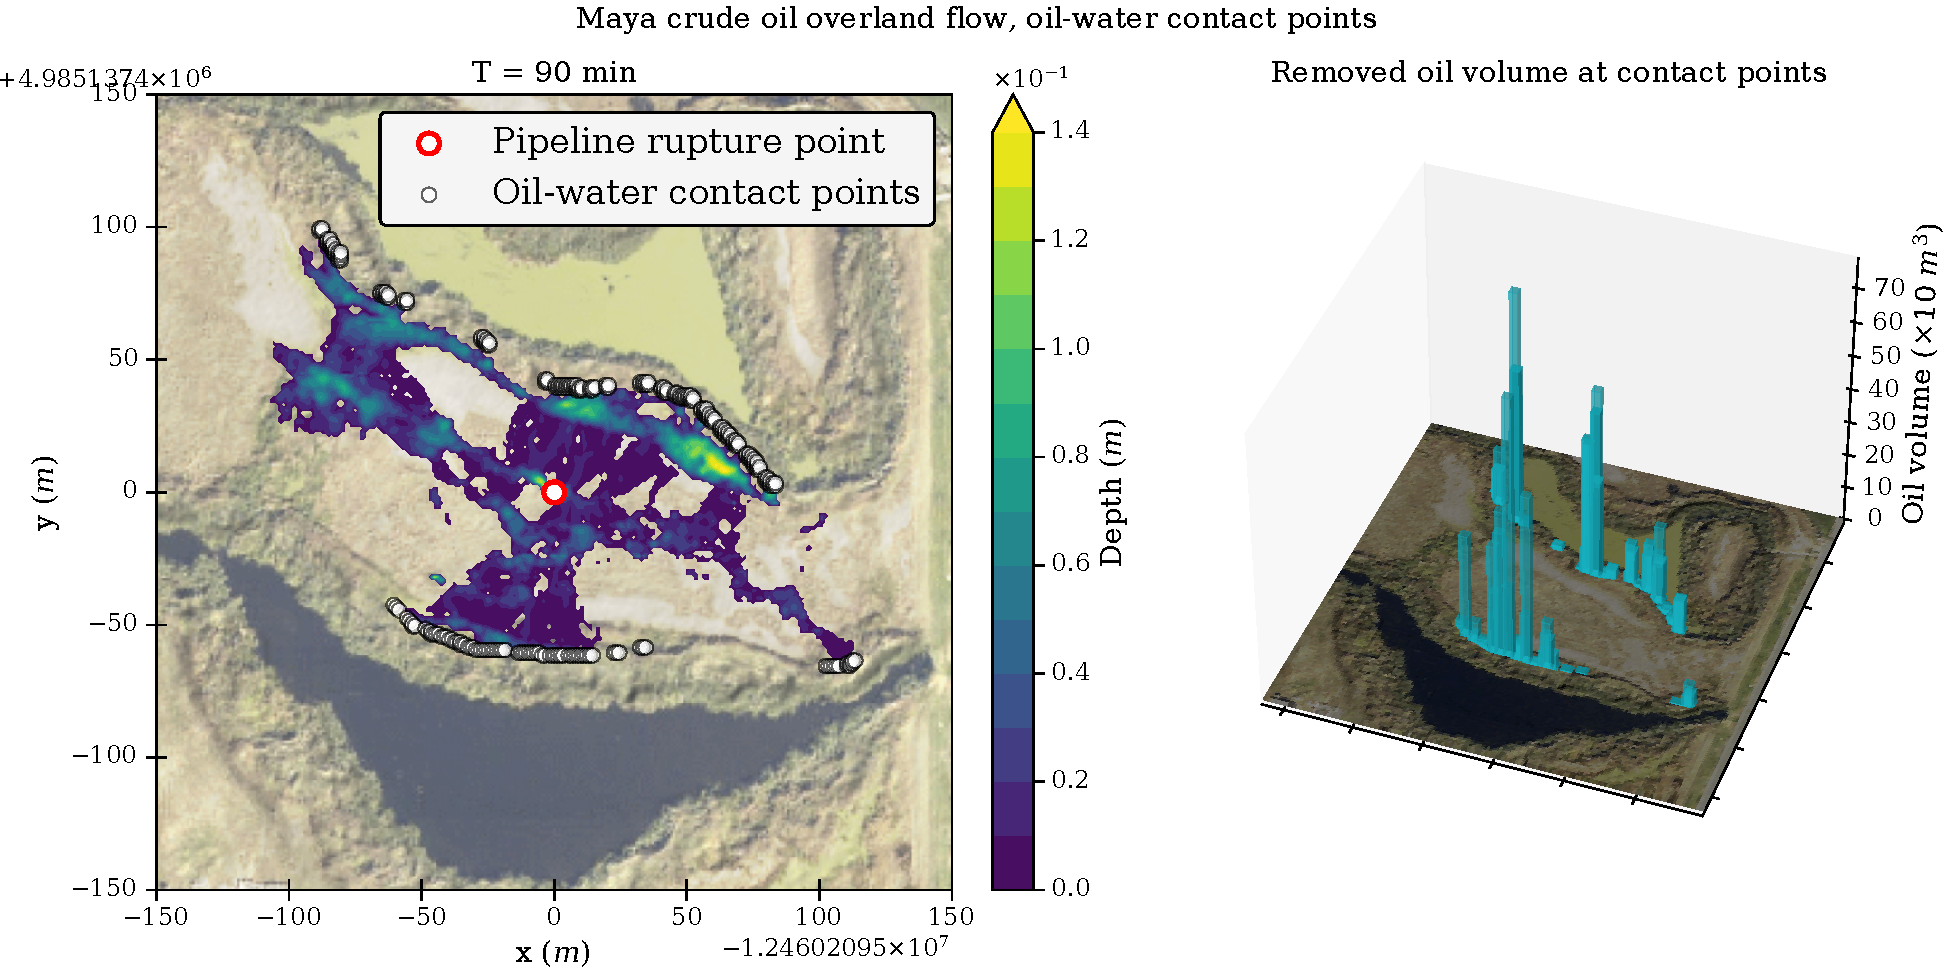
\includegraphics[width=\textwidth]{landspill-maya-hydro}
    \caption{%
        Maya crude oil in contact with water bodies. %
        \geoclawlandspill{} only simulates oil flow above land and does not have hydrographic transport analysis. %
        However, whenever oil flow encounters in-land water bodies, \geoclawlandspill{} records the location of the oil-water contact and the time history of the oil volume flowing into water at each contact location.  %
        These data can be used as the boundary conditions in other third-party hydrographic transport simulation software.%
    }\label{fig:landspill-maya-hydro}
\end{figure*}
% vim:ft=tex:


\section{Discussion} \label{sec:discussion}

Among many different models, those that calculate friction coefficients with one single formula are more suitable than others in terms of numerical simulations.
Pipe and open-channel flows usually have three major flow regimes: 1) laminar flow, 2) smooth turbulent flow, in which surface roughness has no influence, and 3) fully-rough turbulent flow, in which surface roughness plays a key role.
Two transition regimes exist between laminar and smooth turbulent flows and between smooth fully-rough turbulent flows.

All friction models are more or less depending on experimental data fitted onto 1D closed-pipe experiments.

\section{Conclusions} \label{sec:conclusion}

\section*{Software availability}

\section*{Acknowledgment}


% bibliography using biblatex
\sloppy % allow latex to adjust space size so hyphenated words can be fewer
\printbibliography
\fussy % revert the behavior of \sloppy

%% bibliography using natbib; apa style
%\bibliographystyle{apalike}
%\bibliography{reference}

\end{document}
% vim:ft=tex
